\documentclass{article}
%\documentclass[journal]{IEEEtran}
%\documentclass{report}
%\documentclass{ActaOulu}

\usepackage[pdftex,bookmarks=true]{hyperref}
\usepackage[pdftex]{graphicx}
\usepackage[utf8]{inputenc}
\usepackage{cite}
\usepackage{amsmath}

\begin{document}

\title{Charge Collection Efficiency Measurement on Strip Sensors with the Alibava readout system}
\author{Arne-Rasmus Dr\"ager}

\maketitle

\begin{abstract}
In this exercise the charge collection (CC) efficiency of strip sensors are supposed to be determined. The alibava system provides an analog readout of all channels of a strip detector, thus providing the collected charge resulting from a traversing particle. The result should be to measure the degradation of the collected charge as a result of radiation damage. This note gives an introduction to the setup along with a brief explanation of how to operate it.
%The alibava setup can be used to measure the influence of radiation on silicon strip detectors. This note gives an introduction to the setup and a brief explanation how to use it.
\end{abstract}


%\chapter{First Chapter}

\section{Introduction}

High energy particle experiments demand very powerful colliders with high instantaneous luminosities. In order to operate detectors at this high intensities new materials have to be developed that withstand very harsh radiation conditions. The alibava setup is one important setup in the chain of developing new radiation hard silicon strip detectors for the CMS experiments, the so-called phase 2 upgrade. The setup can be used to measure the charge induced by surpassing particles from a $\sideset{^{90}}{}{\mathop{\mathrm{Sr}(\beta)}}$ source or a laser at different temperatures, and different voltages. Because of the increase of leakage current due to irradiation the sensors needs to be cooled to $ -20\,^{\circ}\mathrm{C} $ which is the expected operation temperature of the HL-LHC CMS detector. Further information about the principle operation of Si-detectors can be found in Ref. \cite{Silicon_Microstrip_dectectors_anna_peisert}\cite{Alibava}. The analysis is done using a c++ software called ROOT. A comprehensive tutorial can be found at \cite{ROOT_Tutorial}.
\section{The Setup}
In order to start the measurement process, eight devices need to be turned on before starting the alibava software. All devices are listed in table \ref{tab:devices} and are shown in figure \ref{fig:MainUnits}\ref{fig:InsideTheBox}\ref{fig:CurrentAndVoltageTrigger}\ref{fig:Picture3}.
\begin{table}[htb]
\begin{center}
    \begin{tabular}{|l|l|l|}
        \hline
    No. & Device Name        & Function    \\  \hline
        1 & Keithley 6517A        & Voltage supply and picoamperemeter (multimeter)         \\
        2 & Ortec Model 401B        & Power for scintillator trigger        \\
        3 & TDK-Lambda            & Voltage supply for the peltier element         \\
        4 & Keithley 2700        & Temperature monitor          \\
        5 & Relay box            & Relay box for the setup         \\
        6 & Alibava            & Alibava mother-board         \\
        7 & OWIS            & Driver for the linear stage         \\
        8 & Landa            & Heat exchanger for the peltier element (chiller)         \\
        9 & Two valves            & Dry air supply (optional need for temperatures < dew-point) \\
        \hline

    \end{tabular}
\caption{Table of all devices that need to be turned on.}
\end{center}
\label{tab:devices}
\end{table}
The detector to be measured is fixed and wire-bonded on a so-called daughter-board which consists of two readout chips and periphery. Fig.\ref{fig:InsideTheBox} shows a picture of a sensor on a daughter-board installed in the cold box. Three cables need to be connected: The power supply for the bias voltage , the heat sensor (round cable) and the ribbon cable connecting the daughter-board to the alibava mother-board.
Since a $\sideset{^{90}}{}{\mathop{\mathrm{Sr}(\beta)}}$ source is a radioactive substance the supervisor has to be present when a measurement is performed. (Use the 100MBk source for faster data gathering.)
After turning on all devices and opening the dry air valves (optional if cooling below room temperature) the alibava control software may be started (The password for the computer is: beetle11/09-03).
\newline
\mbox{Make sure: NEVER TURN OF THE PC OR INSTALL ANY UPDATES!!!}
\newline
Start the alibava control program with the conf file:
\newline
 .dist/Debug/GNU-Linux-x86/alibava\_control /space/software/devconf.cfg
\newline
(Make sure the humidity usb is not connected!)
Here one can apply bias voltage, heat or cool the sensor, move the table and finally start measuring.
The measurements are than stored in:
\newline
 /space/measurement/\$DeviceName\$/\$DataTime\$/
\newline
\section{Aim of the Exercise}
In order to obtaining of the CC of a strip sensor these tasks need to be fulfilled:
\begin{itemize}
  \item Measurement of the pedestal of a strip sensor
  \item Measurement of the charge deposited by a $\sideset{^{90}}{}{\mathop{\mathrm{Sr}(\beta)}}$ at a certain temperature and voltage
\end{itemize}
The analysis is performed in several steps:
\begin{itemize}
  \item Subtract common mode noise
  \item Use cluster algorithm to find clusters
  \item Obtain a charge distribution
  \item Fit charge distribution with Landau-Gauss
  \item MPV- of Landau = CC
  \item Plot single channel noise
\end{itemize}

\begin{figure}[tbhn]
\begin{center}
\begin{tabular}{cc}
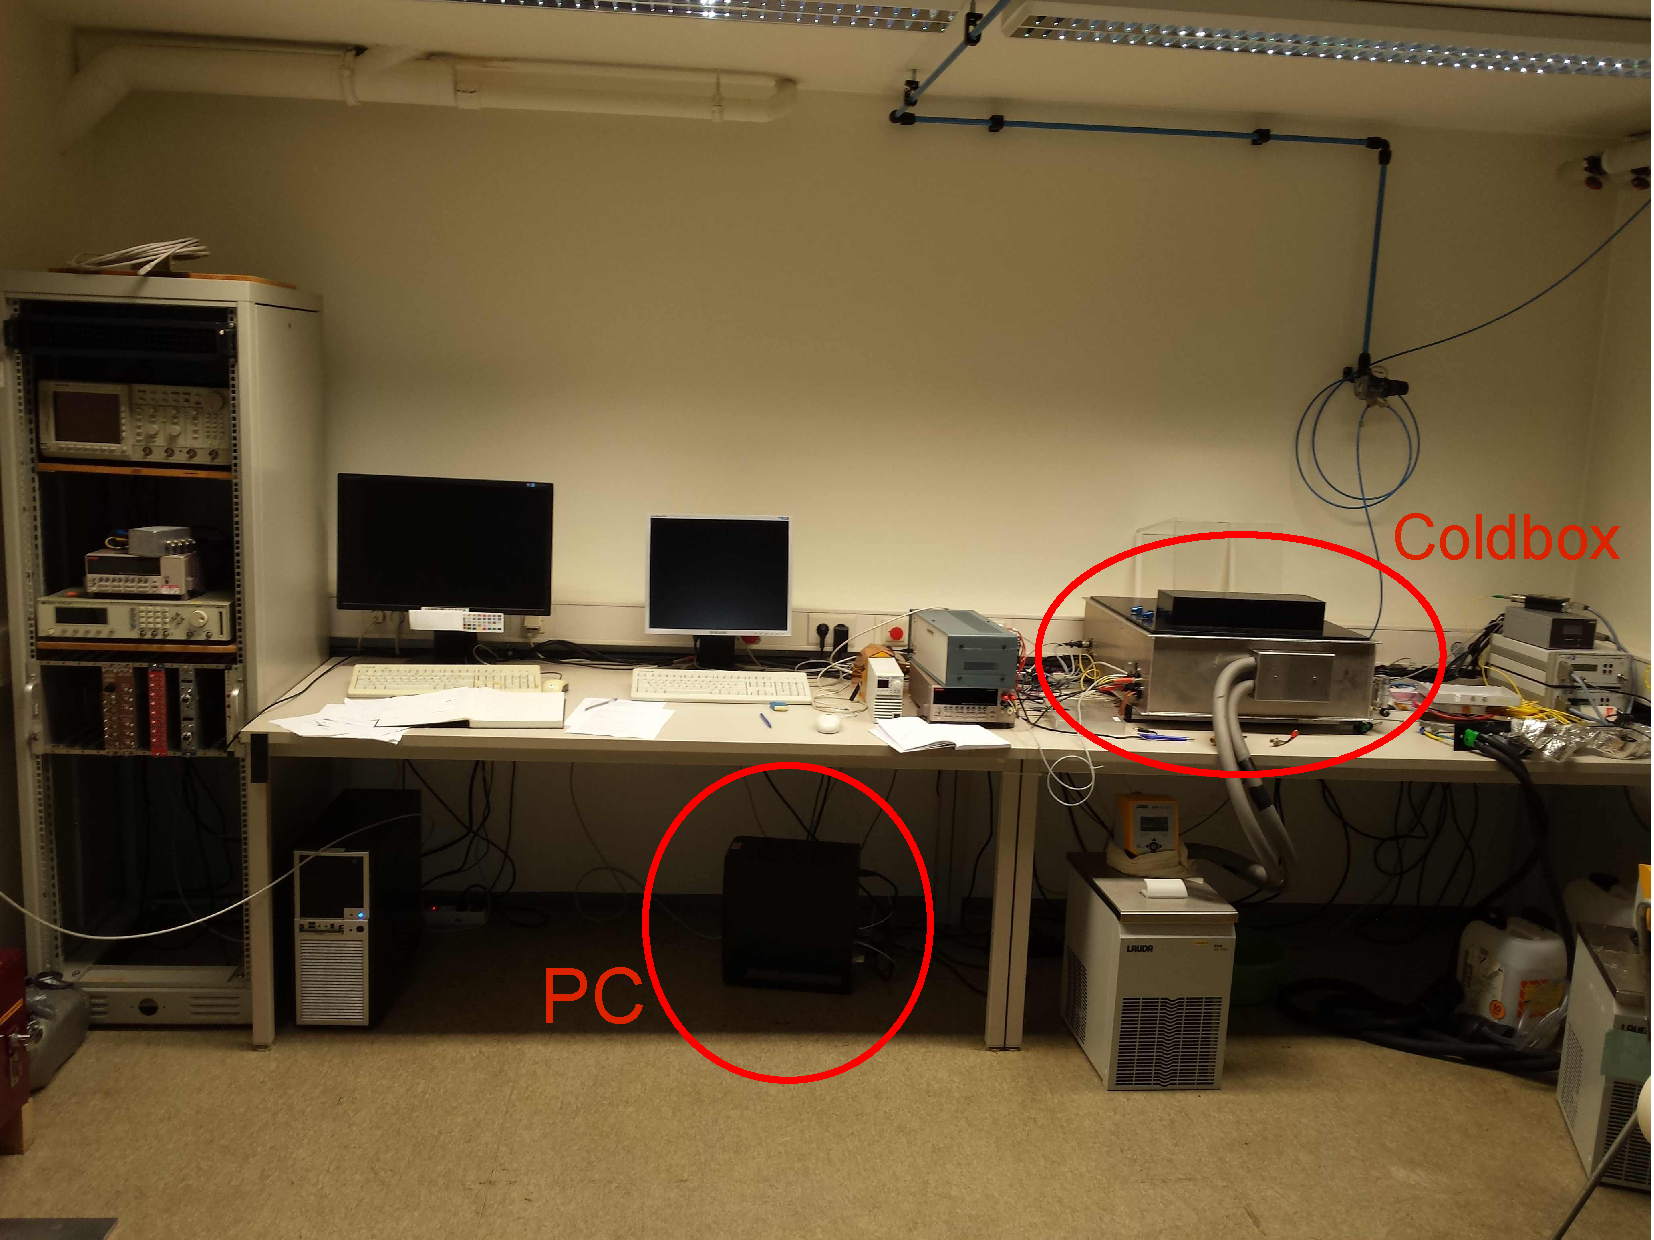
\includegraphics[width=0.45\textwidth]{pictures/FullSetUp.pdf}
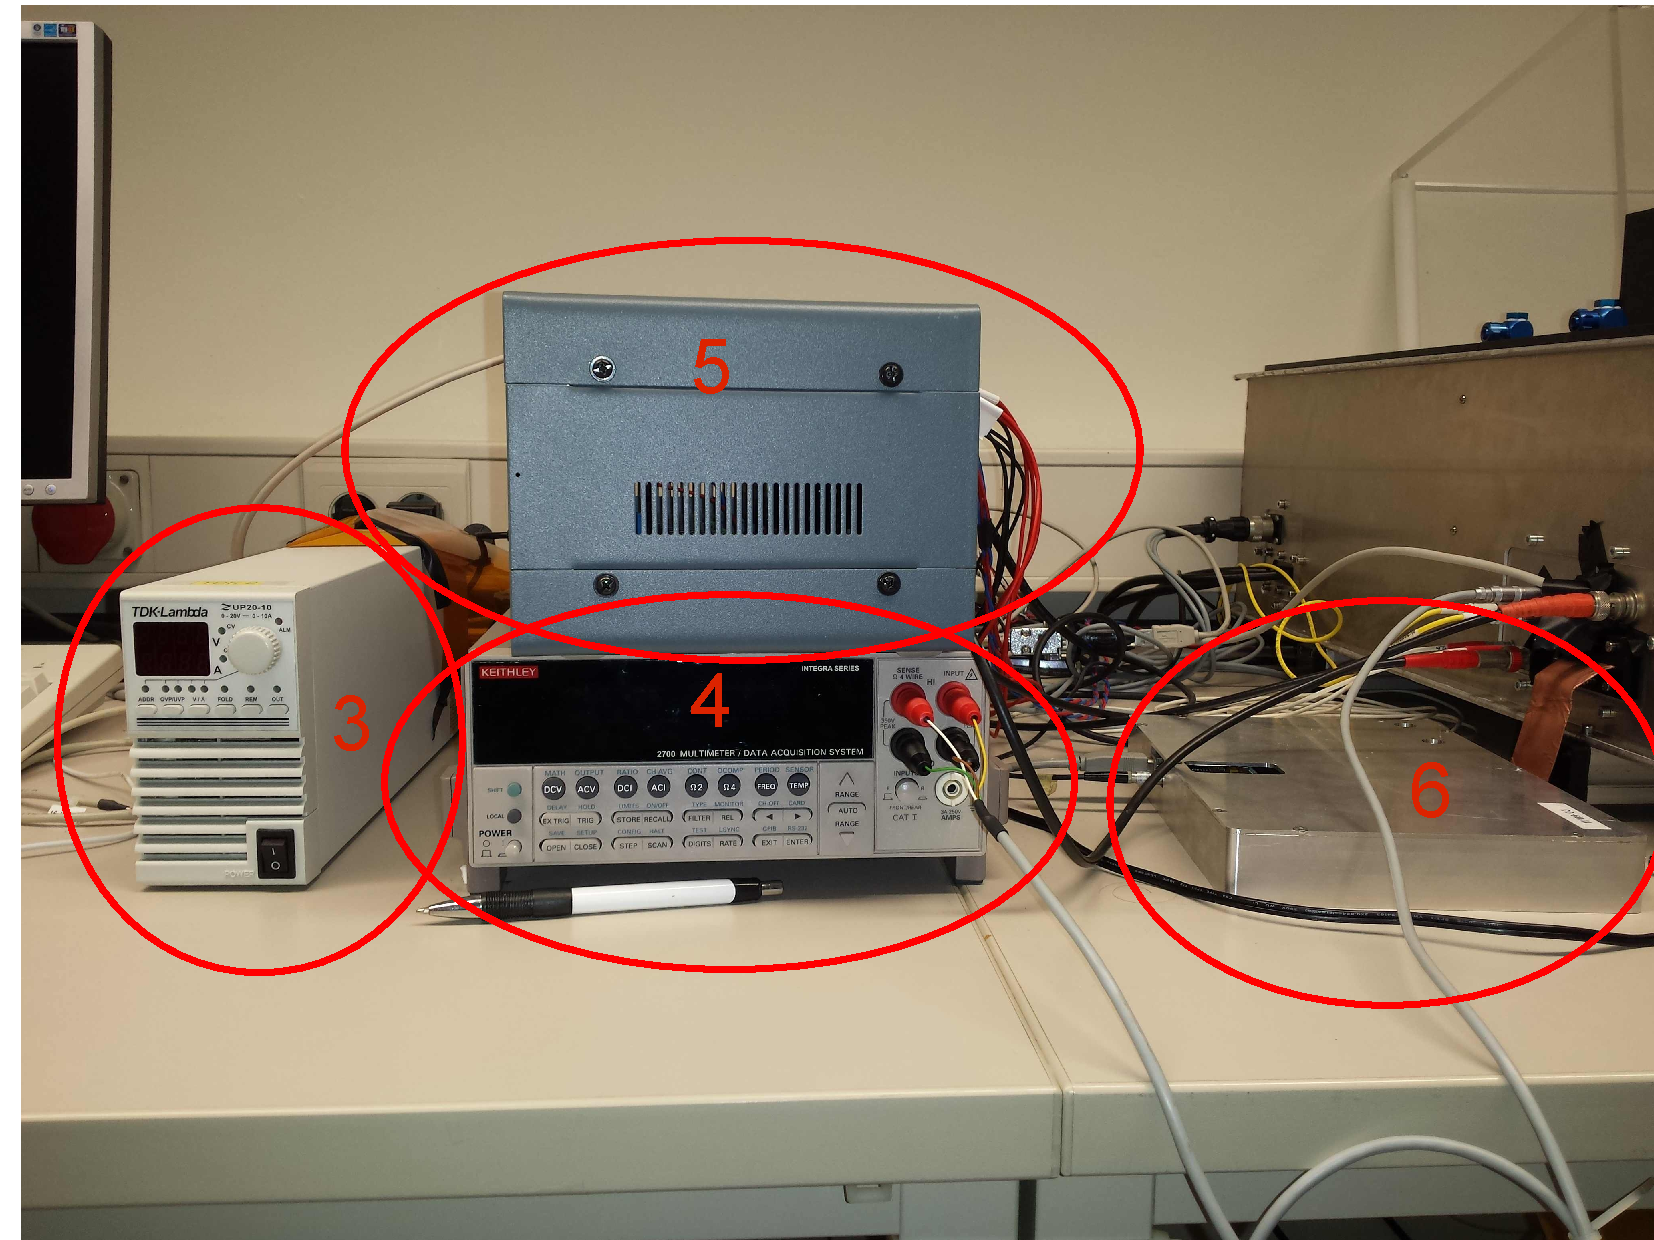
\includegraphics[width=0.45\textwidth]{pictures/3456.pdf}
\end{tabular}
\end{center}
\caption{The left hand side picture shows the full setup while the right hand side shows (from left to right, top to bottom) the Voltage supply for the peltier element (3), relay box(5), temperature monitor(4) and the alibava mother-board(6).}
\label{fig:MainUnits}
\end{figure}
\begin{figure}[tbhn]
\begin{center}
\begin{tabular}{c}
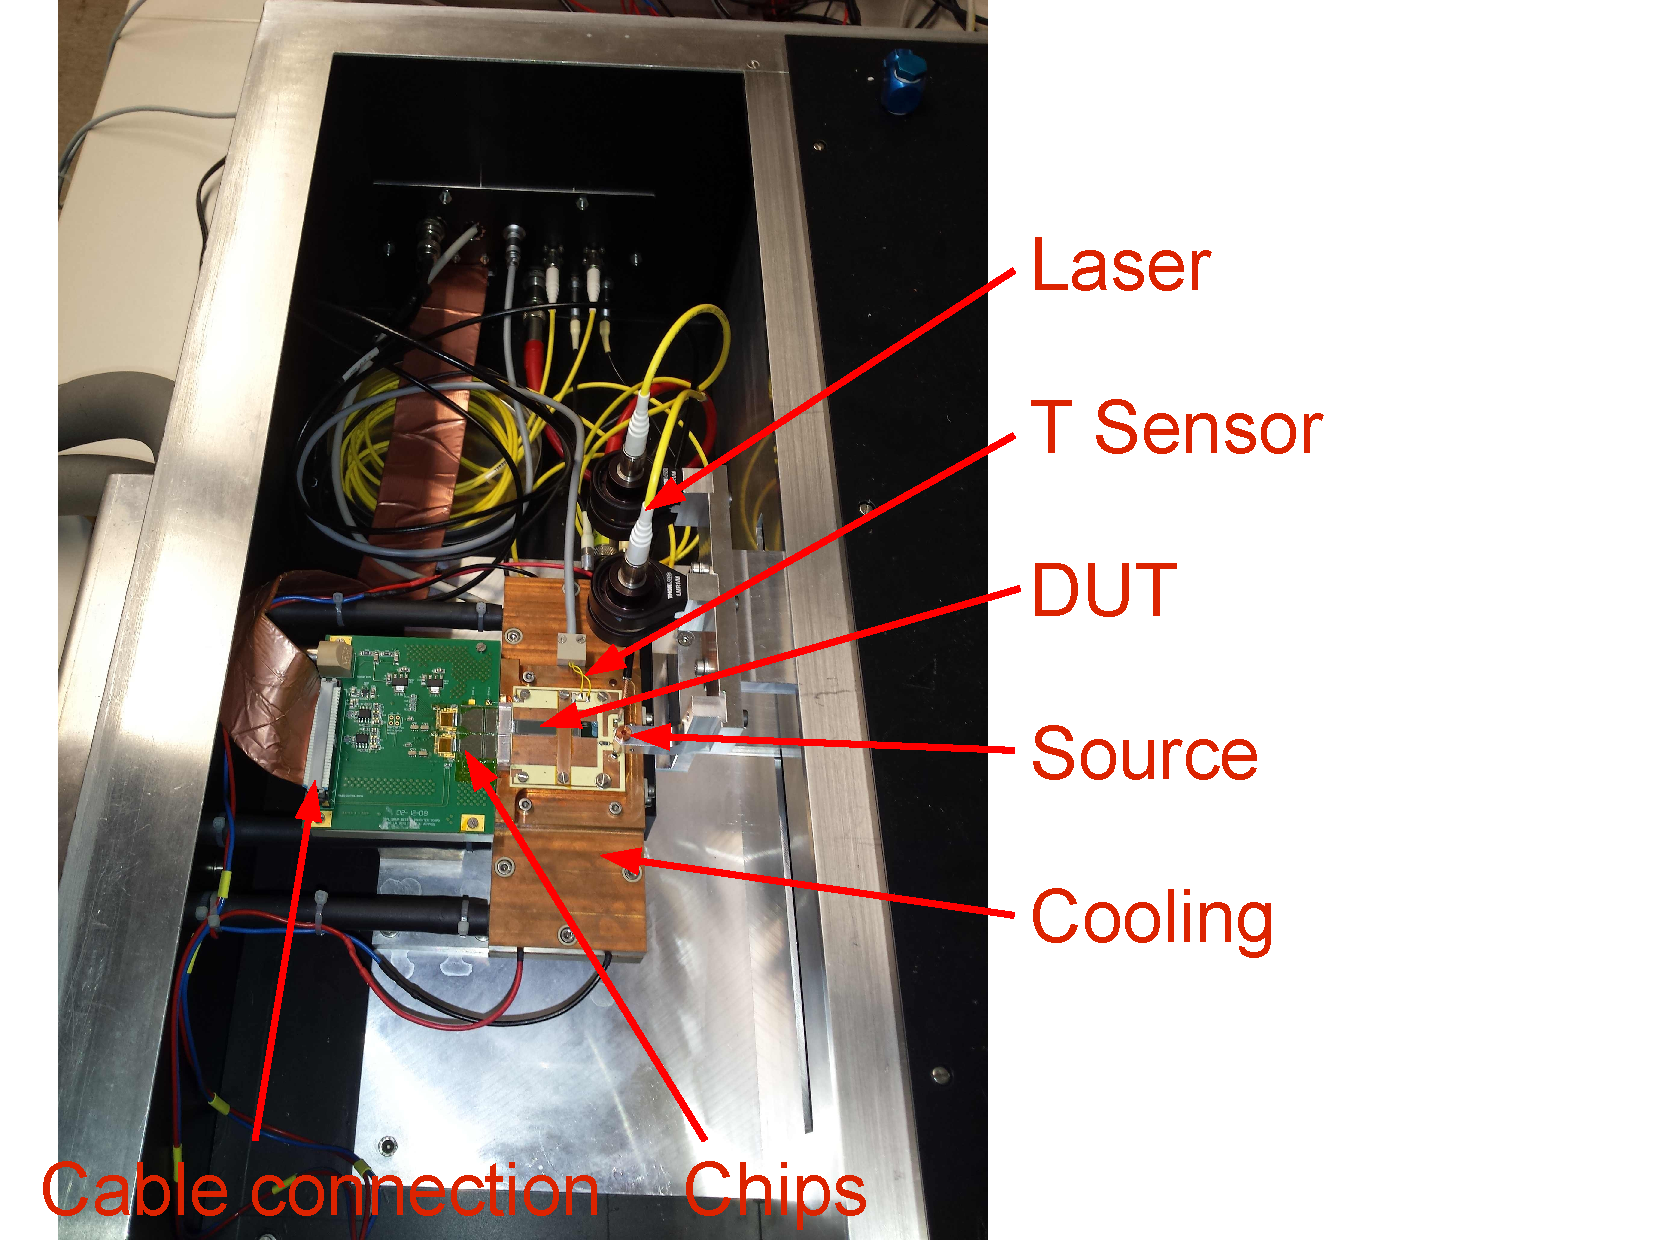
\includegraphics[width=0.98\textwidth]{pictures/InsideTheBox.pdf}
\end{tabular}
\end{center}
\caption{The inside of the light-tide cold box (black) with an alibava daughter-board mounted on a cooling stage can be seen in this picture. The ribbon cable on the left hand side (big flat one) is connected to the alibava mother-board(6) while the gray one with the two yellow end pieces is connected the to the temperature sensor(4) and the black one connects the bias voltage to the detector(1).}
\label{fig:InsideTheBox}
\end{figure}
\begin{figure}[tbhn]
\begin{center}
\begin{tabular}{cc}
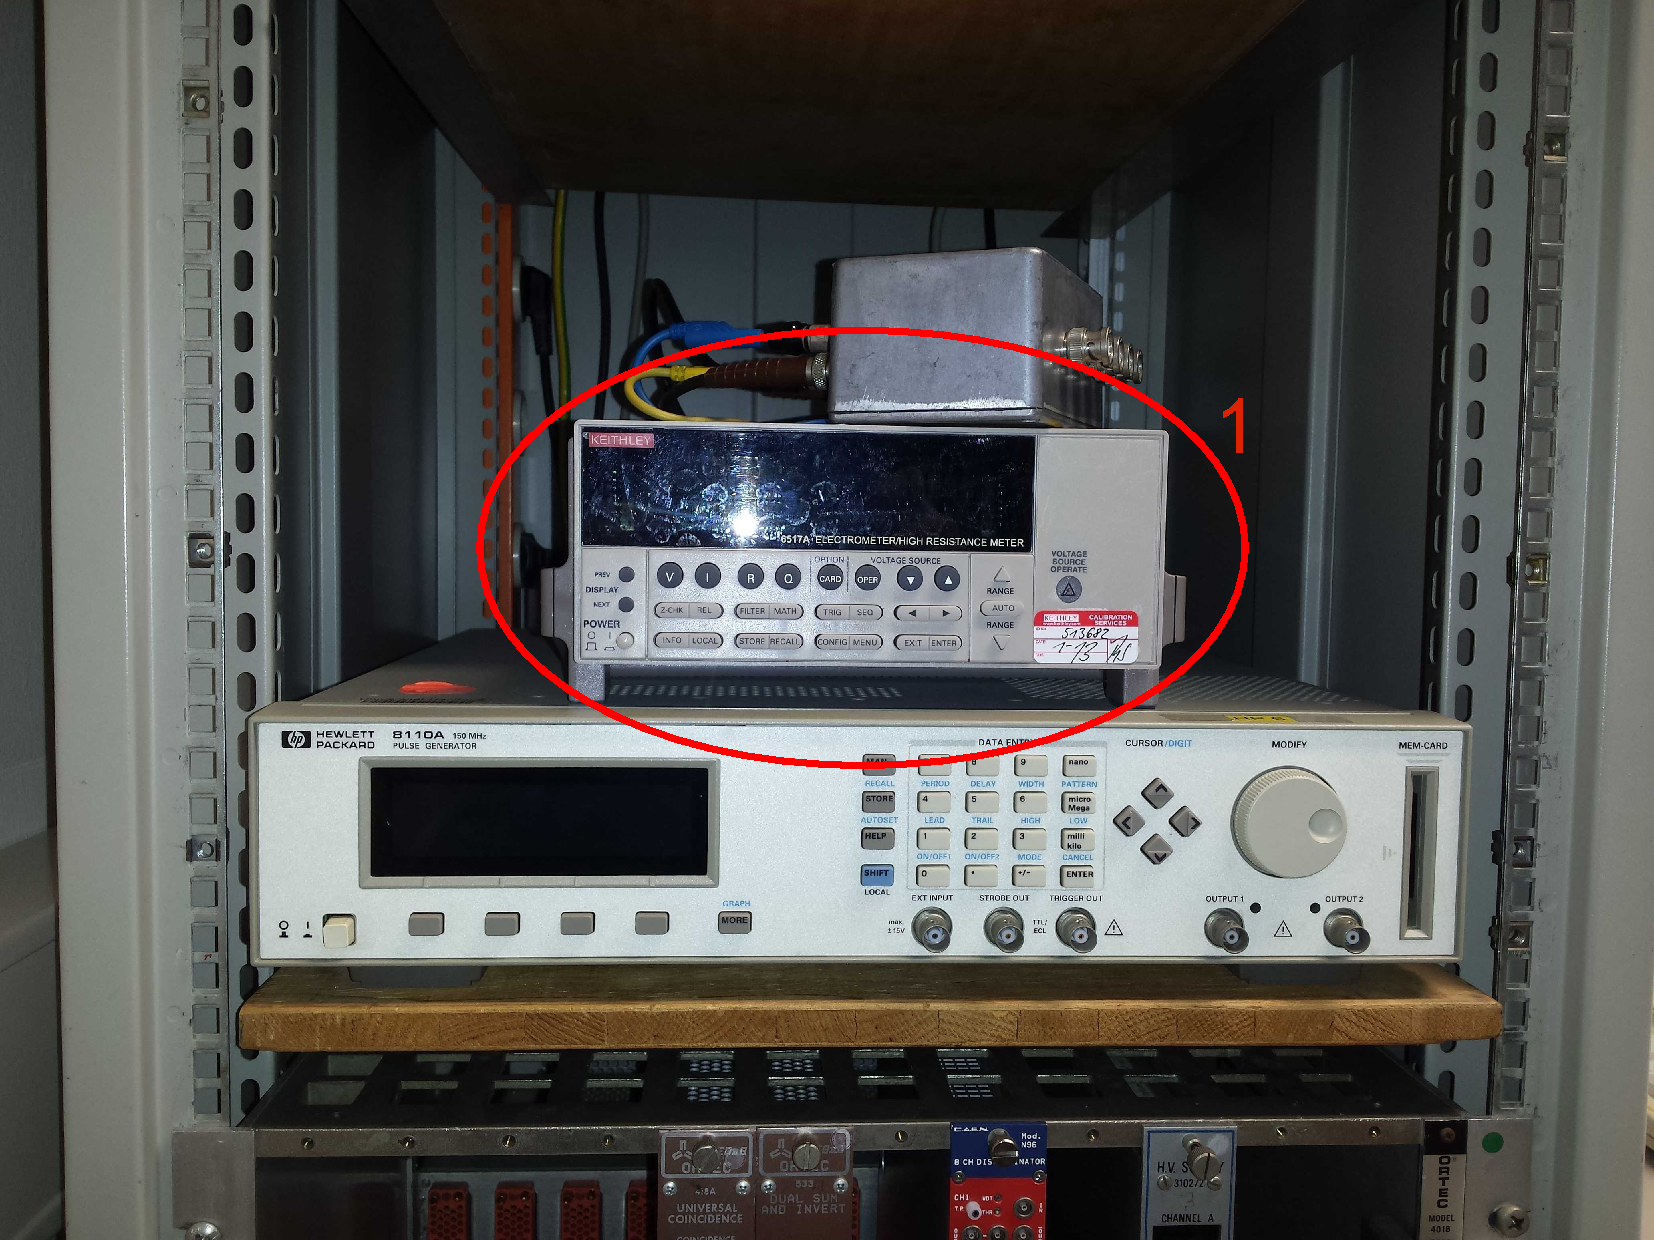
\includegraphics[width=0.48\textwidth]{pictures/1.pdf}
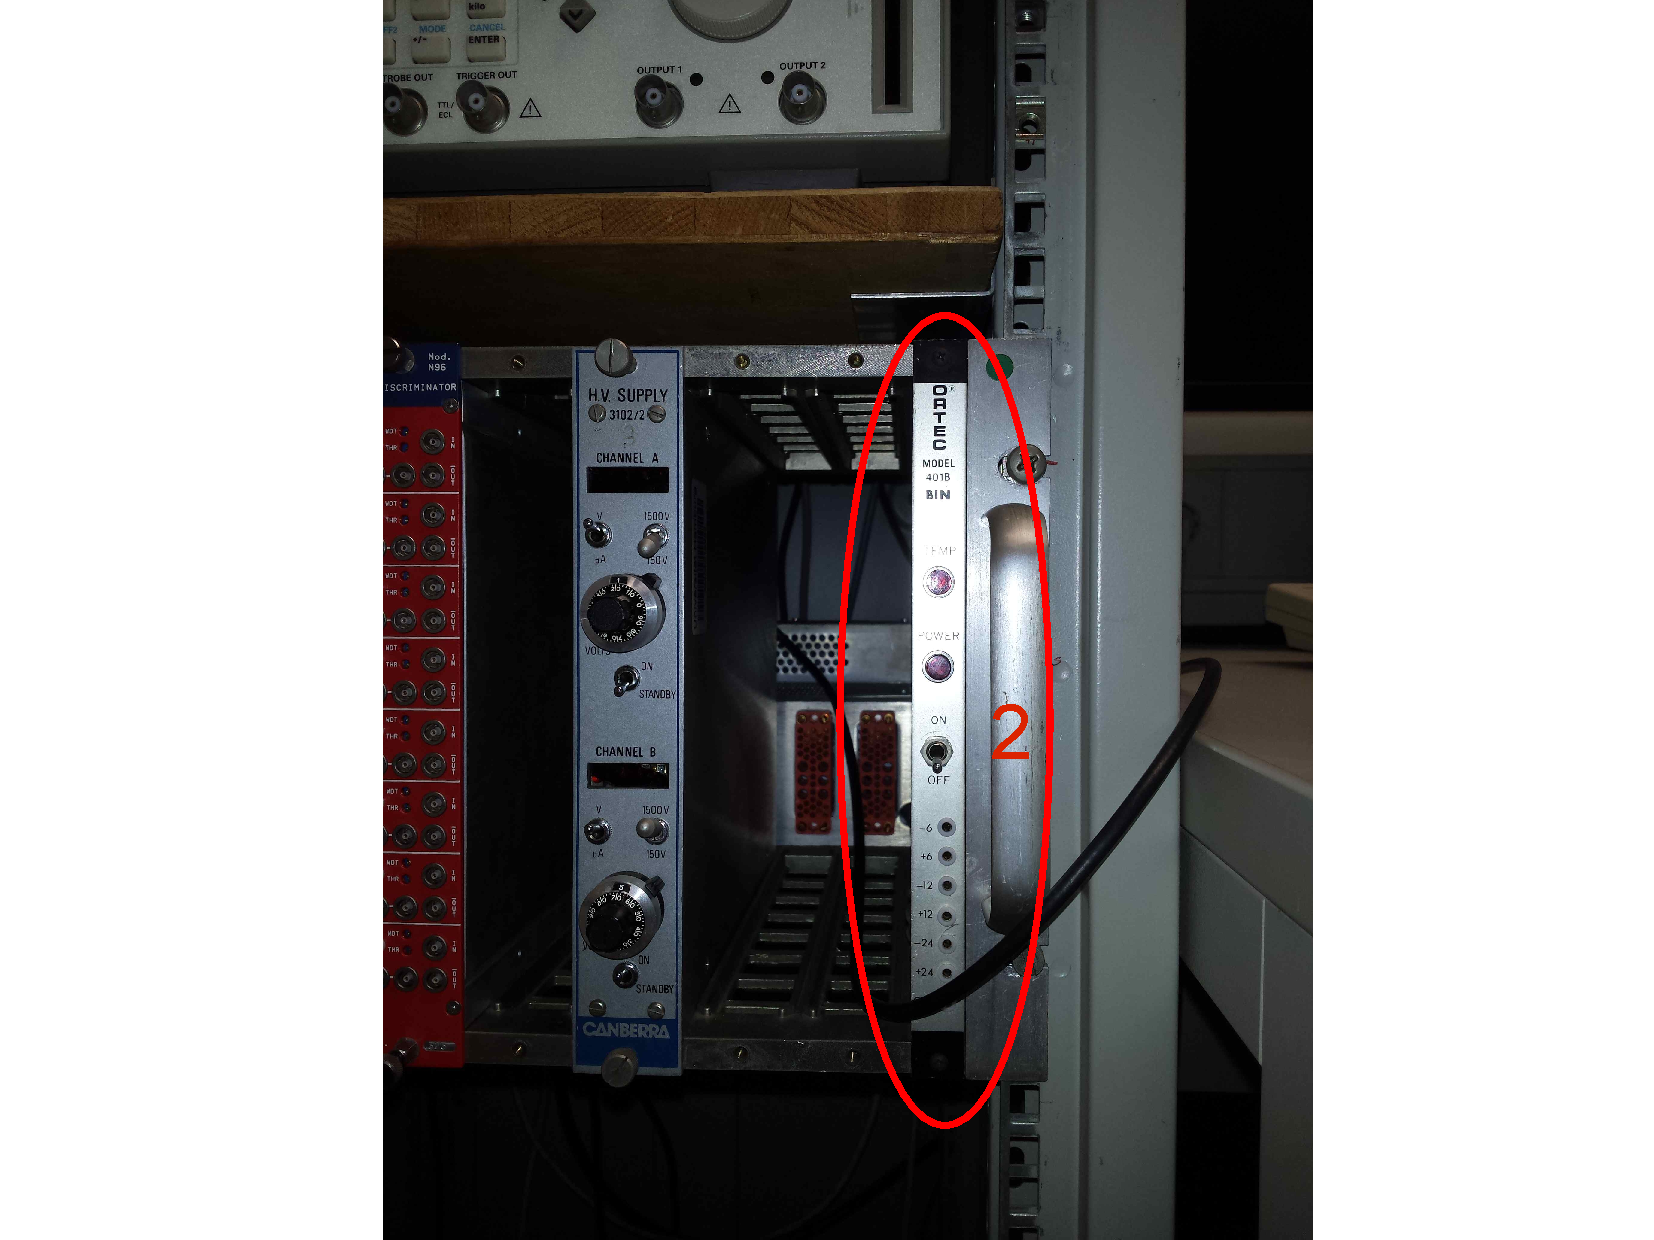
\includegraphics[width=0.48\textwidth]{pictures/2.pdf}
\end{tabular}
\end{center}
\caption{The left hand side picture shows the bias voltage and current supply for the detector(1), while on the right hand side the trigger power supply is shown(2).}
\label{fig:CurrentAndVoltageTrigger}
\end{figure}
\begin{figure}[tbhn]
\begin{center}
\begin{tabular}{cc}
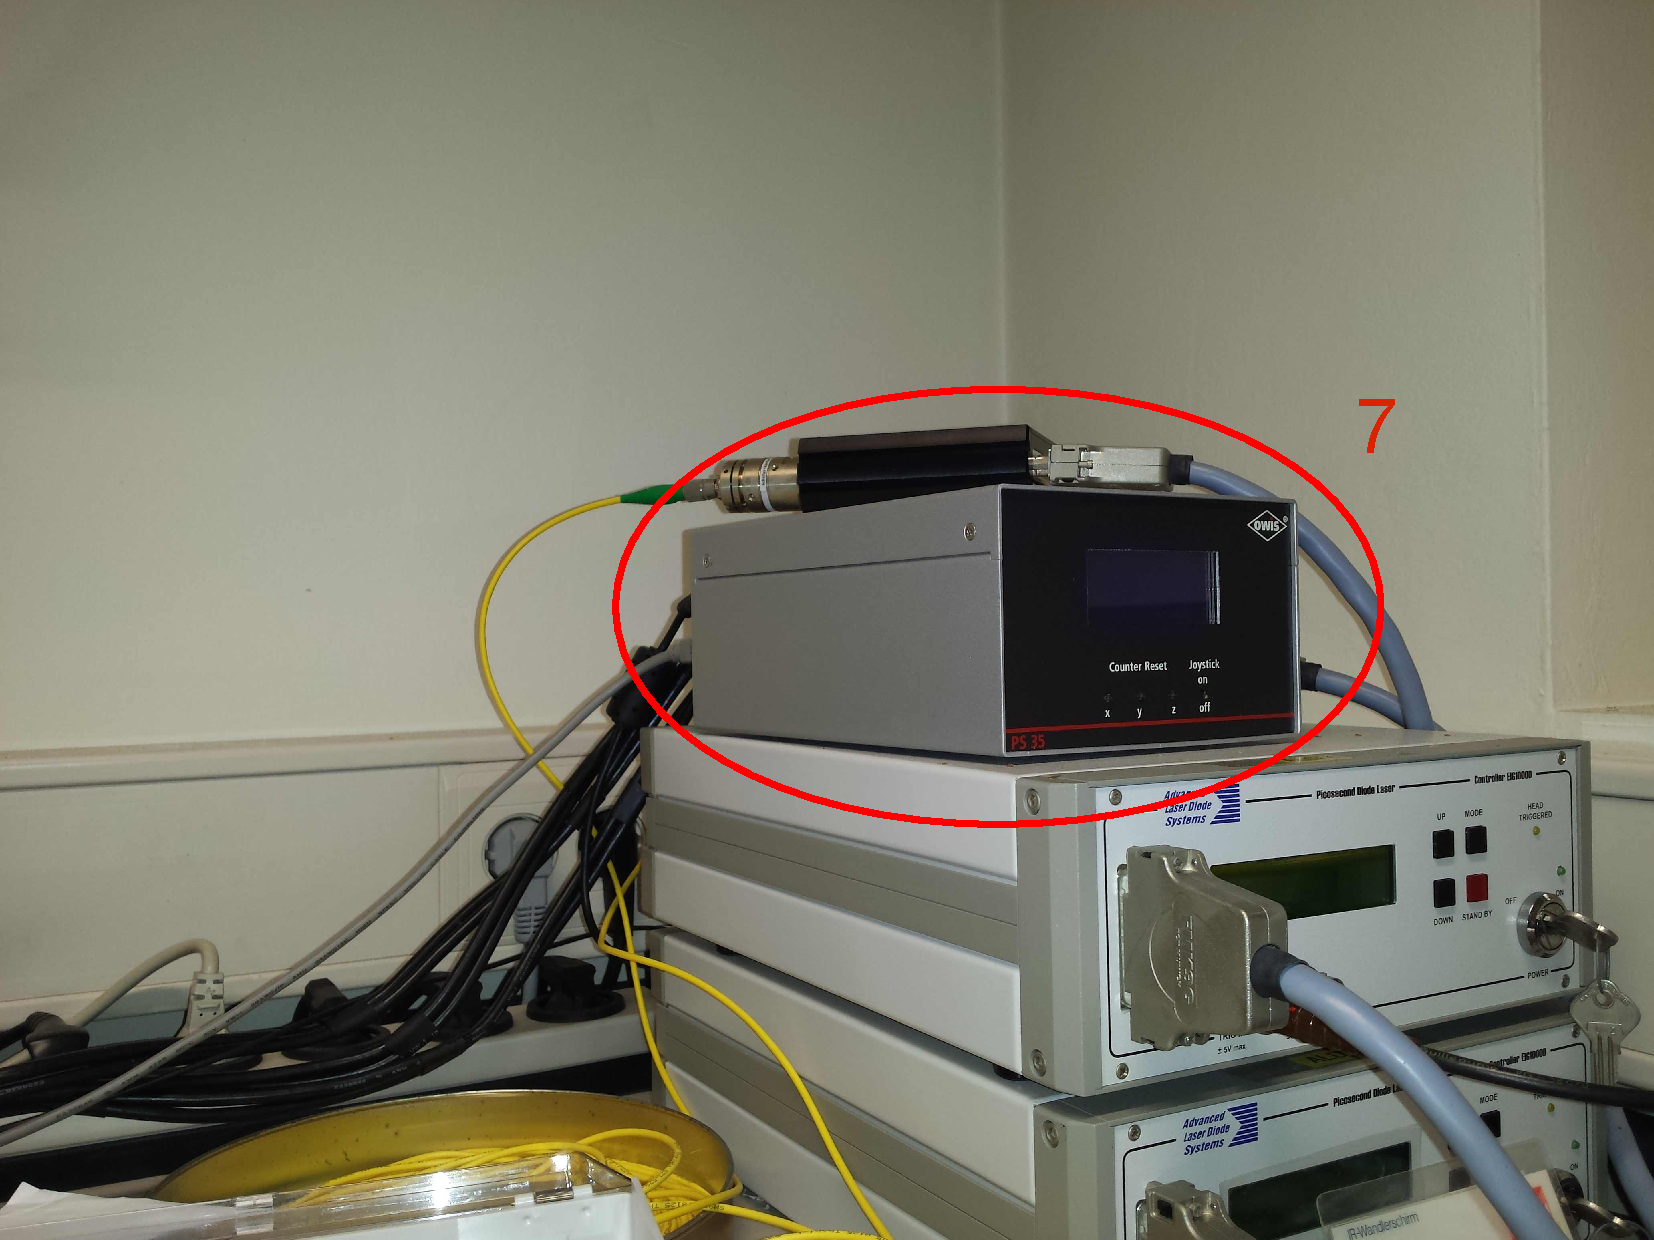
\includegraphics[width=0.31\textwidth]{pictures/7.pdf}
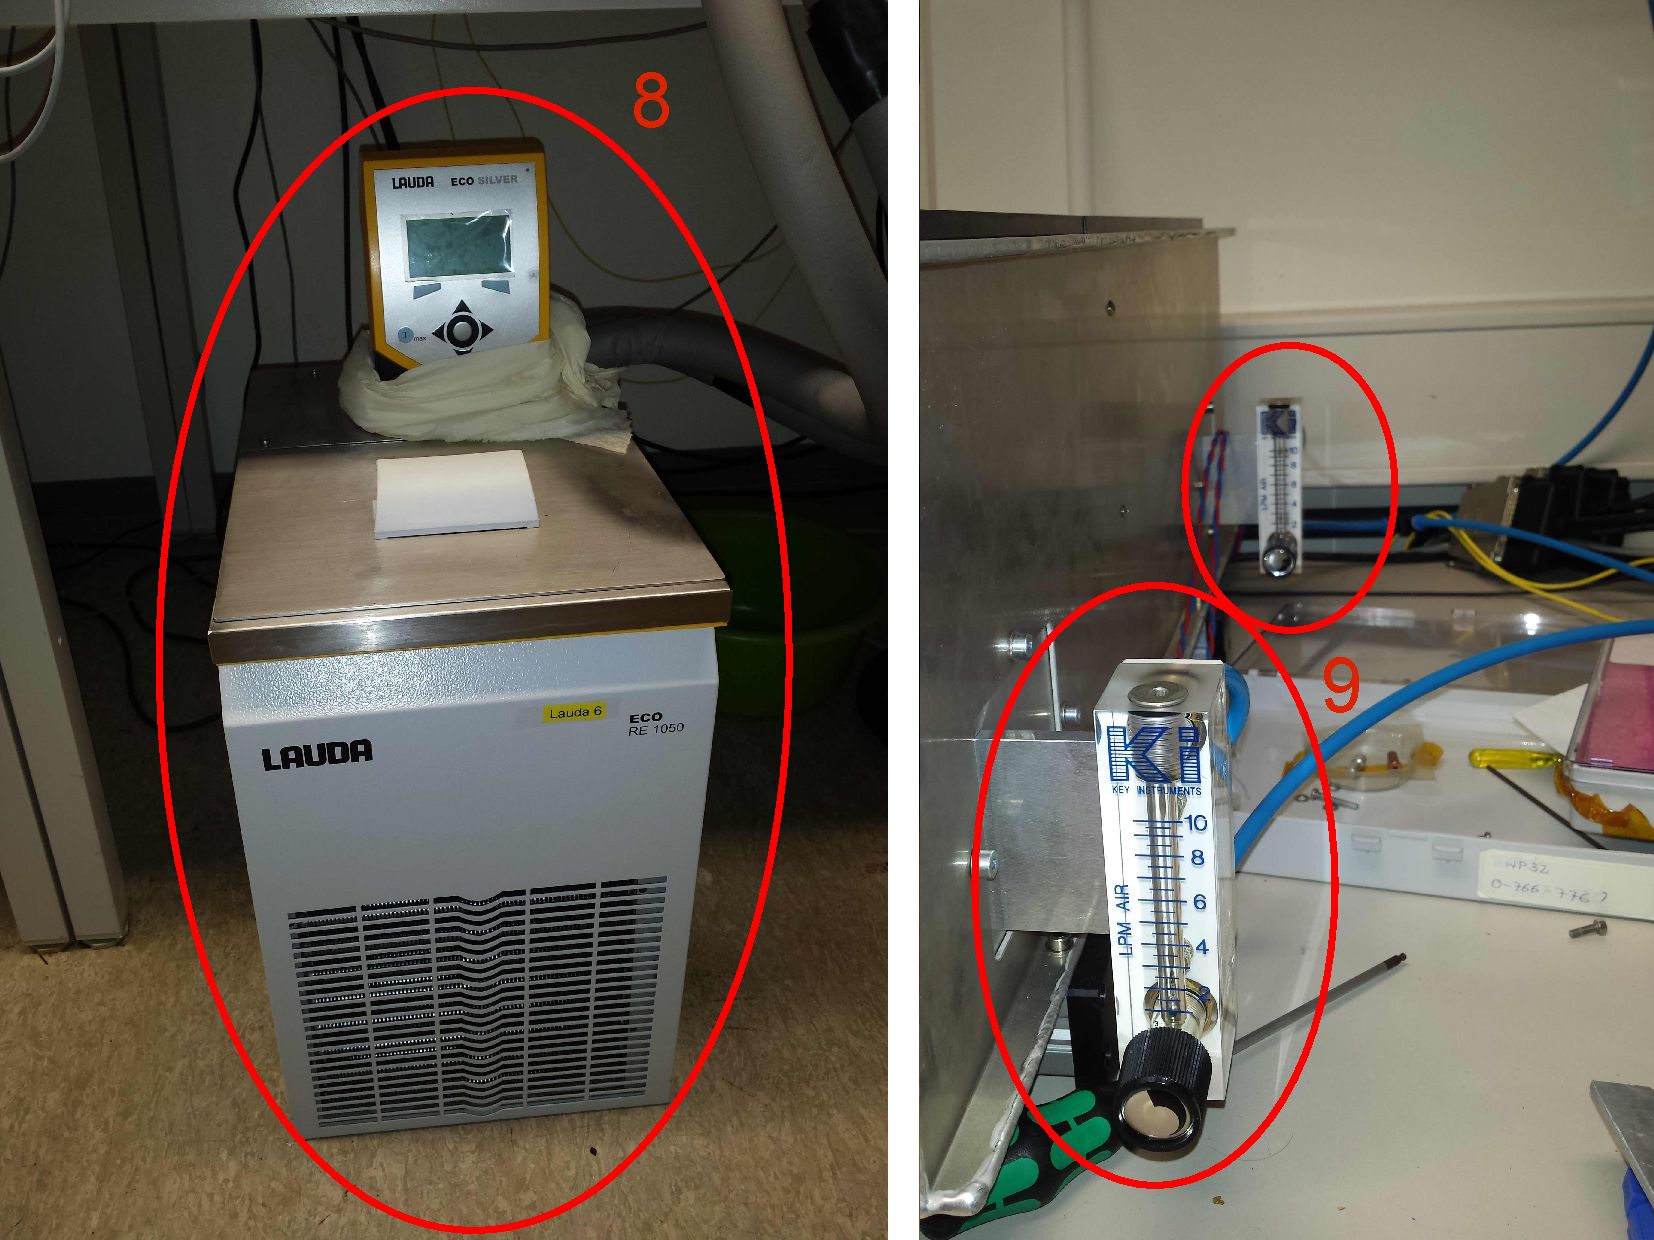
\includegraphics[width=0.62\textwidth]{pictures/89.pdf}
\end{tabular}
\end{center}
\caption{The left hand side picture shows the power supply for the driver of the table(7), in the middle the heat exchanger is shown(8) and on the right the two valves for the dry air supply are visible(9). The numbers in brackets correspond to table \ref{tab:devices}. }
\label{fig:Picture3}
\end{figure}

\bibliography{Master}{}
\bibliographystyle{plain}


\end{document}
